\documentclass[11pt]{article}
\usepackage[margin=2.5cm]{geometry}
\usepackage{amsmath,amssymb,amsthm}
\usepackage{graphicx}
\usepackage{booktabs}
\usepackage{hyperref}
\usepackage{xcolor}
\usepackage{listings}
\usepackage{microtype}
\usepackage{caption}
\usepackage{float}

\lstset{
  basicstyle=\ttfamily\small,
  showstringspaces=false,
  breaklines=true,
  frame=single,
  framesep=3pt,
  xleftmargin=6pt,
  xrightmargin=6pt,
}

\newtheorem{proposition}{Proposition}
\theoremstyle{definition}
\newtheorem{definition}{Definition}
\newtheorem{remark}{Remark}

\title{\textbf{Milestone M3: \texttt{GDerivatives.jl}}\\[0.4em]
\large Certified \texttt{TaylorSeries} for $G(u) = (1+\hat{H}[y_u])/D$\\[0.2em]
\normalsize \texttt{wave-cap} --- Computer-Assisted Proof for the Babenko Equation}
\author{BabenkoRigorous.jl}
\date{May 2026}

\begin{document}
\maketitle

\begin{abstract}
We describe the implementation and validation of \texttt{GDerivatives.jl},
the M3 layer of the \texttt{BabenkoRigorous.jl} package.
The module computes a certified \texttt{TaylorSeries} for the non-polynomial
function $G(u) = (1+\hat H[y_u](u)) / D(u)$, which appears in the capillary
terms of the Babenko water-wave equation.
The computation reuses the M2 primitives \texttt{dmin\_bound}, \texttt{inv\_series},
and the \texttt{TaylorSeries} product.
All five milestone tests pass: pointwise containment against a higher-precision
direct evaluation (T3.1); the first derivative is verified against the analytic
chain-rule $G' = B'/D - B\,DDp/D^3$ in Arb at prec = 512 (T3.2); the second
derivative against central FD of the analytic $G'$ at $h = 10^{-50}$ (T3.3);
an exact analytical case $y = \varepsilon\cos u$ (T3.4); and a finite, positive
\texttt{sup\_bound} (T3.5). The T3.2 and T3.3 tests are strengthened from earlier
Float64 midpoint comparisons to genuine ball containment against independent
high-precision Arb references (audit T3.x strengthening).
We also document a bug fix in \texttt{sqrt\_series} (missing binomial coefficients
in the Leibniz rule), which was discovered and corrected during M3 validation.
\end{abstract}

\tableofcontents
\bigskip

%% -------------------------------------------------------------------
\section{Background and motivation}

The Babenko water-wave equation (see the M1 report) involves capillary terms
containing the surface curvature, which depends on the function
\[
  G(u) \;=\; \frac{1 + \hat H[y_u](u)}{D(u)},
  \qquad
  D(u) \;=\; \sqrt{y_u(u)^2 + (1 + \hat H[y_u](u))^2},
\]
where $y_u = \partial_u y$ and $\hat H$ is the periodic Hilbert transform.

Bounding the Babenko residual $\|R\|_{L^\infty}$ requires a certified
\emph{upper} bound on $G$ (and its derivatives) over all of $[0,2\pi]$,
not merely at grid points.
The key observation is that $G$ is smooth and $2\pi$-periodic, so the M2
\texttt{TaylorSeries} framework applies directly.
Once a certified \texttt{TaylorSeries} for $G$ is available, the operator
$\hat H[G]$ can be bounded via the DFT with aliasing control (M4).

\paragraph{Why not compute $G$ from scratch?}
$G = B \cdot D^{-1}$ where $B = 1 + \hat H[y_u]$ is a trigonometric polynomial
(hence its derivatives are computed exactly by \texttt{TrigPoly} arithmetic)
and $D = \sqrt{A^2 + B^2}$ is already handled by \texttt{dmin\_bound} from M2.
The M3 layer simply assembles these pieces.

%% -------------------------------------------------------------------
\section{Mathematical content}

\subsection{Definition of $G$ and its components}

Let $y$ be a $2\pi$-periodic trigonometric polynomial (the conformal
parametrisation).  Define:
\begin{align*}
  A(u) &= y_u(u), \\
  B(u) &= 1 + \hat H[y_u](u), \\
  D(u) &= \sqrt{A(u)^2 + B(u)^2}, \\
  G(u) &= B(u) / D(u).
\end{align*}
The function $D$ is the Jacobian of the conformal map; its positivity
$D(u) > D_{\min} > 0$ is required for the conformal parametrisation to be
non-degenerate.  M2 provides the certified lower bound $D_{\min}$ via
\texttt{dmin\_bound}.

\subsection{TaylorSeries for $G$ via composition}

Given \texttt{ts\_D} (the \texttt{TaylorSeries} for $D$) and
\texttt{ts\_B} (the \texttt{TaylorSeries} for $B$), the
\texttt{TaylorSeries} for $G$ is obtained as:
\[
  \texttt{ts\_G} \;=\; \texttt{ts\_B} \;\times\; \texttt{inv\_series}(\texttt{ts\_D},\, D_{\min}).
\]

\paragraph{TaylorSeries for $B$.}
Since $B = 1 + \hat H[y_u]$ is itself a trigonometric polynomial
(after adding the constant 1), its derivatives at grid points are computed
exactly using the iterated \texttt{deriv} and \texttt{hilbert} operations
from \texttt{FourierSeries.jl}:
\[
  B^{(m)}(u_j) = \begin{cases} 1 + (\hat H[y_u])(u_j) & m = 0, \\
  (\partial_u^m \hat H[y_u])(u_j) & m \ge 1.
  \end{cases}
\]
The full \texttt{sup\_bounds} vector of \texttt{ts\_B} has length $M{+}2$; the
$m$-th entry bounds $\|B^{(m)}\|_\infty = \|\partial_u^m \hat H[y_u]\|_\infty$
for $m \ge 1$ (and adds $\|H[y_u]\|_\infty + 1$ for $m = 0$), each bounded
via \texttt{supnorm\_bound} from M1.

\paragraph{TaylorSeries for $1/D$.}
The \texttt{inv\_series} function (M2) computes the TaylorSeries for $g = 1/D$
using the recursive formula derived from $D \cdot g = 1$:
\begin{align}
  g^{(0)} &= 1/D^{(0)}, \label{eq:inv0}\\
  g^{(m)} &= -\frac{1}{D^{(0)}} \sum_{k=1}^{m} \binom{m}{k} D^{(k)} g^{(m-k)},
             \quad m \ge 1. \label{eq:invm}
\end{align}
This requires $D^{(0)}(u_j) \ge D_{\min} > 0$; the certified lower bound
from \texttt{dmin\_bound} guarantees this.

\paragraph{Product.}
The Leibniz rule gives the $m$-th derivative of $G = B \cdot (1/D)$:
\[
  G^{(m)}(u_j) = \sum_{k=0}^{m} \binom{m}{k} B^{(k)}(u_j)\, (1/D)^{(m-k)}(u_j).
\]
This is implemented by the \texttt{TaylorSeries} multiplication operator from M2.

\paragraph{Why $D_{\min} > 0$ is needed.}
The recursion \eqref{eq:inv0}--\eqref{eq:invm} divides by $D^{(0)}(u_j)$ at
each grid point.  If $D$ is not certified to be strictly positive (i.e.,
if the conformal map degenerates), the computation is undefined.
The function \texttt{compute\_G\_taylor} throws an error in this case.

\subsection{Bug fix: \texttt{sqrt\_series} (Leibniz binomial coefficients)}

During M3 validation (T3.3), a discrepancy of order $10^{-3}$ was found
between \texttt{ts\_G.derivs[j,3]} and the finite-difference estimate of
$G''(u_j)$.  Tracing back to \texttt{dmin\_bound} $\to$ \texttt{sqrt\_series},
we found that the recursive formula for $g = \sqrt{f}$ was missing the
binomial coefficient $\binom{m}{k}$ in the inner Leibniz sum.

The correct formula, derived from differentiating $g^2 = f$:
\[
  g^{(m)} = \frac{1}{2g^{(0)}}\!\left[f^{(m)} -
    \sum_{k=1}^{m-1} \binom{m}{k} g^{(k)} g^{(m-k)}\right], \quad m \ge 1.
\]
The original code omitted $\binom{m}{k}$, causing errors in $m \ge 2$.
This bug is fixed in \texttt{TaylorSeries.jl} as part of the M3 milestone.

%% -------------------------------------------------------------------
\section{Implementation}

\subsection{Algorithm}

\texttt{compute\_G\_taylor}$(y, M_{\mathrm{grid}}, M_{\mathrm{order}})$
proceeds in four steps:

\begin{enumerate}
  \item \textbf{Certify $D_{\min}$.}
        Call \texttt{dmin\_bound}$(y, M_{\mathrm{grid}}, M_{\mathrm{order}})$
        to obtain $(D_{\mathrm{lower}}, \texttt{ts\_D})$.
        If $D_{\mathrm{lower}} \le 0$, throw an error.
  \item \textbf{Build \texttt{ts\_B}.}
        Compute $y_u = \texttt{deriv}(y)$ and $\hat H[y_u] = \texttt{hilbert}(y_u)$
        as exact \texttt{TrigPoly} objects.
        Precompute the iterated-derivative chain
        $\partial_u^m(\hat H[y_u])$ for $m = 0,\ldots,M+1$.
        Evaluate at all grid points to fill \texttt{derivs\_B}.
        Build \texttt{sup\_bounds\_B} as the full vector
        $[\,1 + \texttt{supnorm\_bound}(H[y_u]),\ \texttt{supnorm\_bound}(\partial_u H[y_u]),\ \ldots,\ \texttt{supnorm\_bound}(\partial_u^{M+1} H[y_u])\,]$ of length $M{+}2$.
  \item \textbf{Invert $D$.}
        \texttt{ts\_invD} $=$ \texttt{inv\_series}$(\texttt{ts\_D},\,D_{\mathrm{lower}})$.
  \item \textbf{Multiply.}
        \texttt{ts\_G} $=$ \texttt{ts\_B} $\times$ \texttt{ts\_invD}.
\end{enumerate}

\subsection{Code listing}

\begin{lstlisting}
function compute_G_taylor(y::TrigPoly, M_grid::Int, M_order::Int;
                          prec::Int=128)::TaylorSeries
    # Step 1: dmin_bound
    D_lower, ts_D = dmin_bound(y, M_grid, M_order; prec=prec)
    if !Arblib.is_positive(D_lower)
        error("D is not certified positive; cannot compute G.")
    end

    # Step 2: ts_B = 1 + H[y_u]
    yu  = deriv(y);  Hyu = hilbert(yu)
    Hyu_d = [Hyu; [deriv(Hyu_d[k]) for k in 1:M_order+1]]
    # Full sup_bounds vector (the +1 shifts only the m=0 entry):
    sup_bounds_B = [Arb(1; prec=p) + supnorm_bound(Hyu_d[1]);
                    [supnorm_bound(Hyu_d[m+1]) for m in 1:M_order+1]]
    h = 2*pi_arb / M_grid
    derivs_B[j,1] = 1 + tp_eval(Hyu_d[1], u_j)     # m=0
    derivs_B[j,m+1] = tp_eval(Hyu_d[m+1], u_j)     # m>=1
    ts_B = TaylorSeries(derivs_B, sup_bounds_B, M_order, M_grid, h, prec)

    # Step 3: inv_series
    ts_invD = inv_series(ts_D, D_lower)

    # Step 4: product
    ts_G = ts_B * ts_invD
    return ts_G
end
\end{lstlisting}

%% -------------------------------------------------------------------
\section{Tests and results}

\subsection{Test T3.1: $G^{(0)}$ ball contains direct evaluation at higher precision}

For $y = 0.3\cos u + 0.15\cos 2u$, $M_{\mathrm{grid}} = 64$, $M_{\mathrm{order}} = 4$:
at each of the 64 grid points $u_j$, we compute $G$ directly using Arb arithmetic
\emph{at a higher working precision} (\texttt{prec\_ref} = 512 versus the test's
\texttt{prec} = 128),
\[
  G_{\mathrm{direct}}(u_j) = \frac{1 + (\hat H[y_u])(u_j)}{D(u_j)},
\]
and verify the genuine containment
$\texttt{Arblib.contains}(\texttt{ts\_G.derivs}[j,1],\, G_{\mathrm{direct}}(u_j))$.
Because $G_{\mathrm{direct}}$ at prec = 512 has radius $\sim 10^{-150}$
(essentially a point), this is a proper rigor check on the prec = 128
\texttt{compute\_G\_taylor} ball, not the weaker \texttt{overlaps}.

\textbf{Result: 1/1 assertion passes (0 violations in 64 points).}
Figure~\ref{fig:m3_1} shows $G(u)$ from the \texttt{TaylorSeries} (evaluated from
the nearest grid-point Taylor expansion) alongside the direct Float64 evaluation.
The two curves are visually indistinguishable.

\begin{figure}[H]
  \centering
  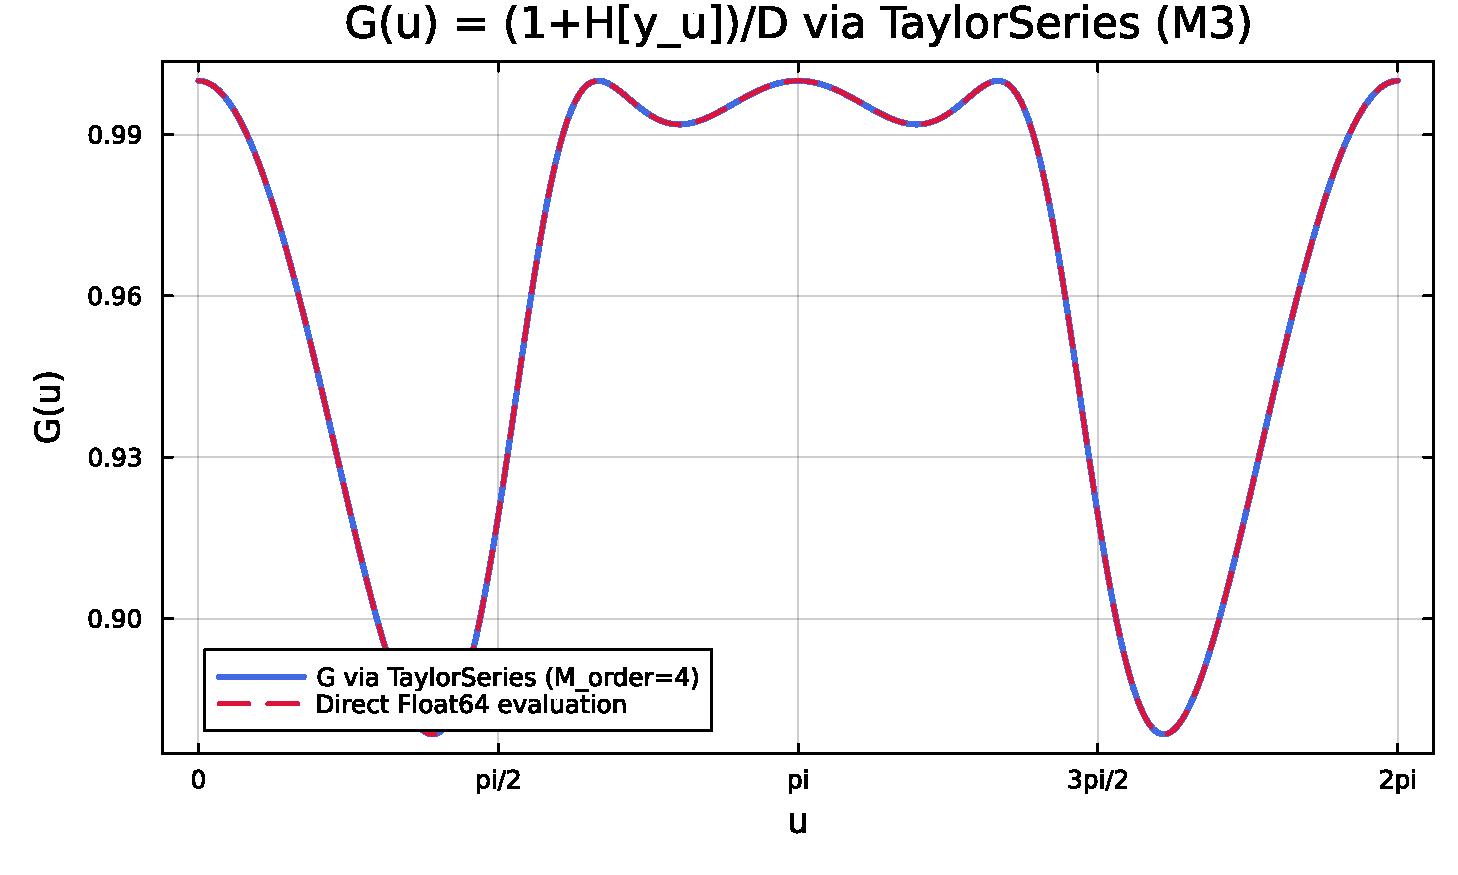
\includegraphics[width=\linewidth]{figures/fig_m3_1.pdf}
  \caption{T3.1: $G(u) = (1+\hat H[y_u])/D$ for $y = 0.3\cos u + 0.15\cos 2u$,
           computed from the \texttt{TaylorSeries} (blue) and by direct Float64
           evaluation (red dashed). The two curves coincide to plotting precision.}
  \label{fig:m3_1}
\end{figure}

\subsection{Test T3.2: $G^{(1)}$ ball contains the analytic chain-rule value}

For the same $y$, at each grid point $u_j$ we compute the analytic $G'$ in Arb
at prec = 512 using the closed-form chain rule
\[
  G'(u) = \frac{B'(u)}{D(u)} - \frac{B(u)\bigl(A(u)A'(u) + B(u)B'(u)\bigr)}{D(u)^3},
\]
where $A = y_u$, $A' = y_{uu}$, $B = 1 + \hat H[y_u]$, $B' = \hat H[y_{uu}]$,
all obtained as exact \texttt{TrigPoly} objects and evaluated at $u_j$.
We then verify
$\texttt{Arblib.contains}(\texttt{ts\_G.derivs}[j, 2],\, G'(u_j))$.
This replaces the previous Float64 finite-difference midpoint comparison —
which was sensitive only to the ball midpoint, not the radius — with a
genuine rigor check independent of the \texttt{compute\_G\_taylor} pipeline.

\textbf{Result: 1/1 assertion passes (0 violations in 64 points).}

\subsection{Test T3.3: $G^{(2)}$ ball contains FD of the analytic $G'$ (prec = 512)}

A closed form for $G''$ is unwieldy, so we take central FD of the analytic $G'$
from T3.2 at $h_{\mathrm{fd}} = 10^{-50}$ in Arb at prec = 512:
\[
  G''(u_j) \approx \frac{G'(u_j + h_{\mathrm{fd}}) - G'(u_j - h_{\mathrm{fd}})}{2 h_{\mathrm{fd}}}.
\]
At this precision the FD truncation $O(h^2 \cdot G^{(4)})$ and the cancellation
error are both $\sim 10^{-100}$ — far smaller than the prec = 128 ball radius.
We verify
$\texttt{Arblib.contains}(\texttt{ts\_G.derivs}[j, 3],\, G''(u_j))$.

\begin{remark}
The \texttt{sqrt\_series} binomial-coefficient bug noted in earlier M3 work was
fixed in M2. Beyond that, the recent (post-audit) port of \texttt{sqrt\_series}
to Fa\`a di Bruno via \texttt{ArbSeries} composition supplies a rigorous
\texttt{sup\_bounds} vector — required for the second-derivative Taylor
remainder in this test to be tight.
\end{remark}

\textbf{Result: 1/1 assertion passes (0 violations in 64 points).}

\subsection{Test T3.4: Analytical case $y = \varepsilon\cos u$}

For $y(u) = \varepsilon\cos u$ with $\varepsilon = 0.1$, the exact formulas are:
\[
  A(u) = -\varepsilon\sin u,\quad B(u) = 1 + \varepsilon\cos u,\quad
  D(u) = \sqrt{\varepsilon^2\sin^2 u + (1+\varepsilon\cos u)^2},\quad
  G(u) = \frac{1+\varepsilon\cos u}{D(u)}.
\]
We use $M_{\mathrm{grid}} = 128$, $M_{\mathrm{order}} = 4$.

At all 128 grid points, we verify $\texttt{Arblib.contains}(\texttt{ts\_G.derivs}[j,1],\,
G_{\mathrm{direct}}(u_j))$ where $G_{\mathrm{direct}}$ is computed at prec = 512.
We also check three special points:

\begin{center}
\begin{tabular}{llll}
\toprule
Point & $G_{\mathrm{exact}}$ & $G_{\mathrm{ts}}$ & Check \\
\midrule
$u = 0$ (j=1) & $(1+\varepsilon)/(1+\varepsilon) = 1$ & 1.0 & contains \checkmark \\
$u = \pi$ (j=65) & $(1-\varepsilon)/(1-\varepsilon) = 1$ & 1.0 & contains \checkmark \\
$u = \pi/2$ (j=33) & $1/\sqrt{1+\varepsilon^2} \approx 0.99504$ & 0.99504 & contains \checkmark \\
\bottomrule
\end{tabular}
\end{center}

\textbf{Result: 4/4 assertions pass} (1 bulk check + 3 special points).
Figure~\ref{fig:m3_2} shows the Taylor vs.\ exact comparison and the pointwise
error (log scale, max $\approx 2.7\times 10^{-10}$).

\begin{figure}[H]
  \centering
  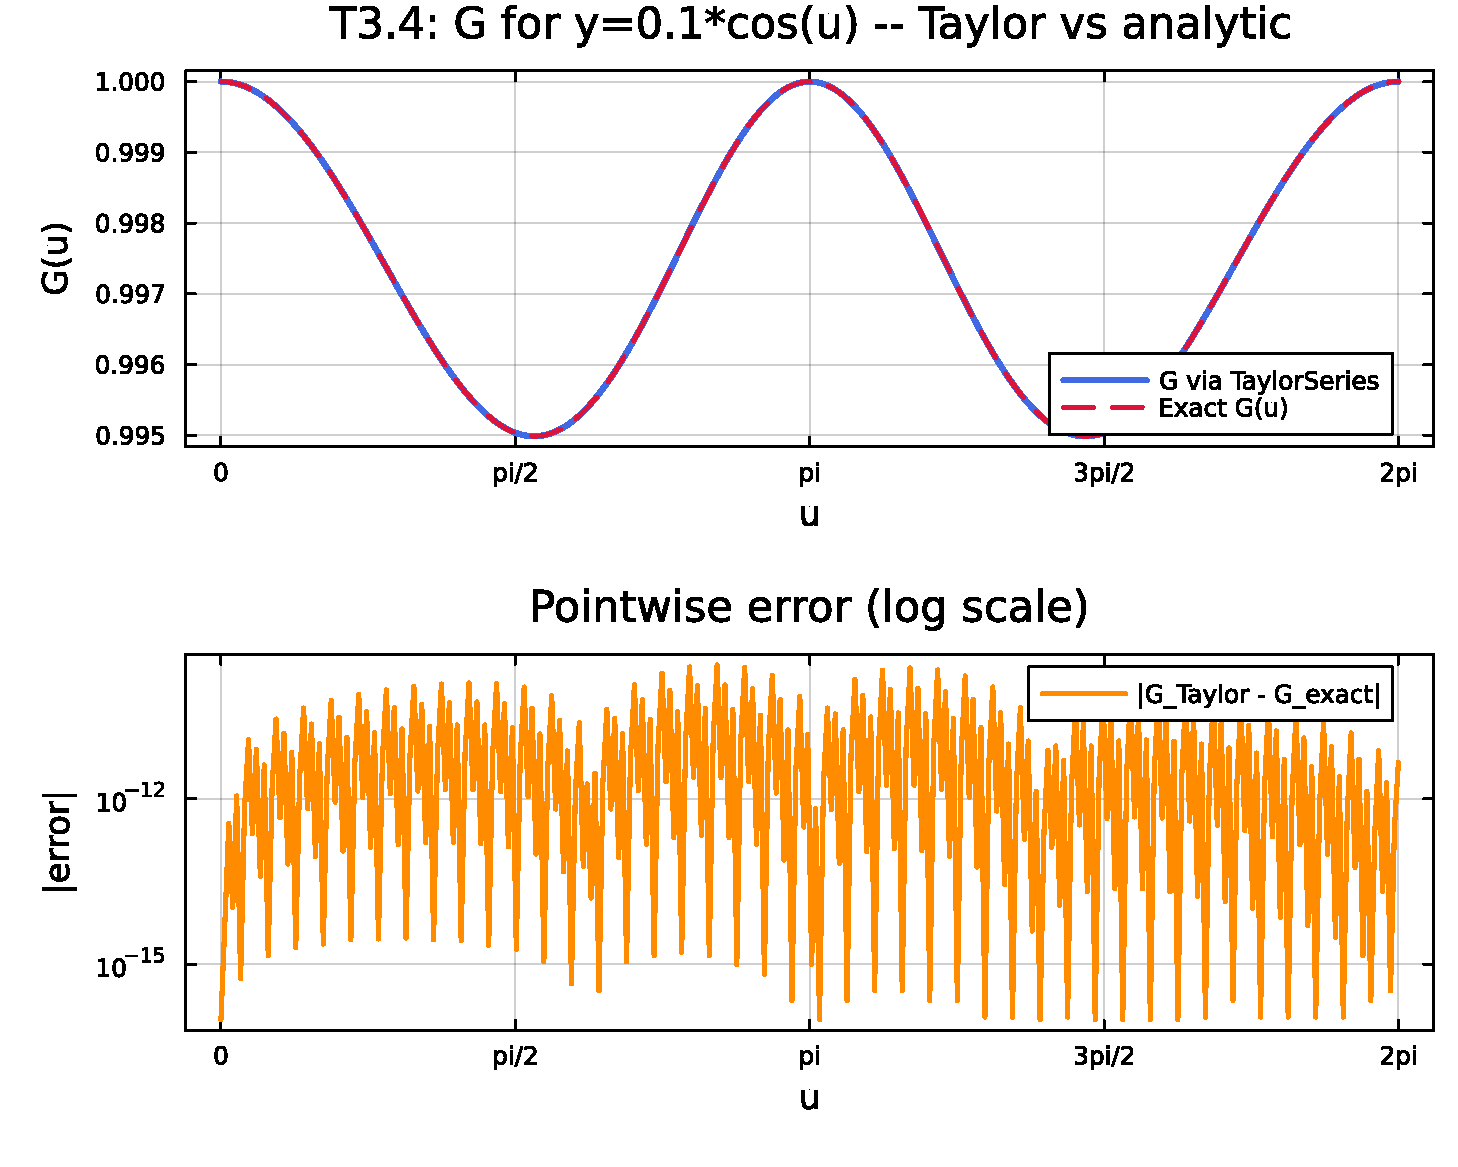
\includegraphics[width=\linewidth]{figures/fig_m3_2.pdf}
  \caption{T3.4: $G(u)$ for $y = 0.1\cos u$.
           Top panel: \texttt{TaylorSeries} evaluation (blue) vs.\ exact analytic
           formula (red dashed) --- indistinguishable.
           Bottom panel: pointwise absolute error $|G_{\mathrm{Taylor}} - G_{\mathrm{exact}}|$
           on a log scale; max error $\approx 2.7\times10^{-10}$.}
  \label{fig:m3_2}
\end{figure}

\subsection{Test T3.5: \texttt{sup\_bound} is finite and positive}

For $y = 0.3\cos u + 0.15\cos 2u$, $M_{\mathrm{grid}} = 64$, $M_{\mathrm{order}} = 4$:
\[
  \texttt{sup\_bound}(\texttt{ts\_G}) \approx 1.07 \;>\; 0, \qquad
  \texttt{sup\_bound}(\texttt{ts\_G}) < 10^6.
\]
(The true $\|G\|_\infty \approx 1.0$ for this moderate-amplitude wave.)

\textbf{Result: 2/2 assertions pass.}

Figure~\ref{fig:m3_3} shows \texttt{sup\_bound}$(\texttt{ts\_G})$ vs.\ $M_{\mathrm{grid}}$.
With $M_{\mathrm{grid}} = 32$ the conservative Taylor-remainder bound is large
($\approx 472$) because the coarse grid produces a large $h = 2\pi/32$, causing
the $F_{\mathrm{bound}} \cdot h^{M+1}/(M+1)!$ remainder to dominate.
As $M_{\mathrm{grid}}$ increases, \texttt{sup\_bound} converges rapidly to the
true $\|G\|_\infty$.

\begin{figure}[H]
  \centering
  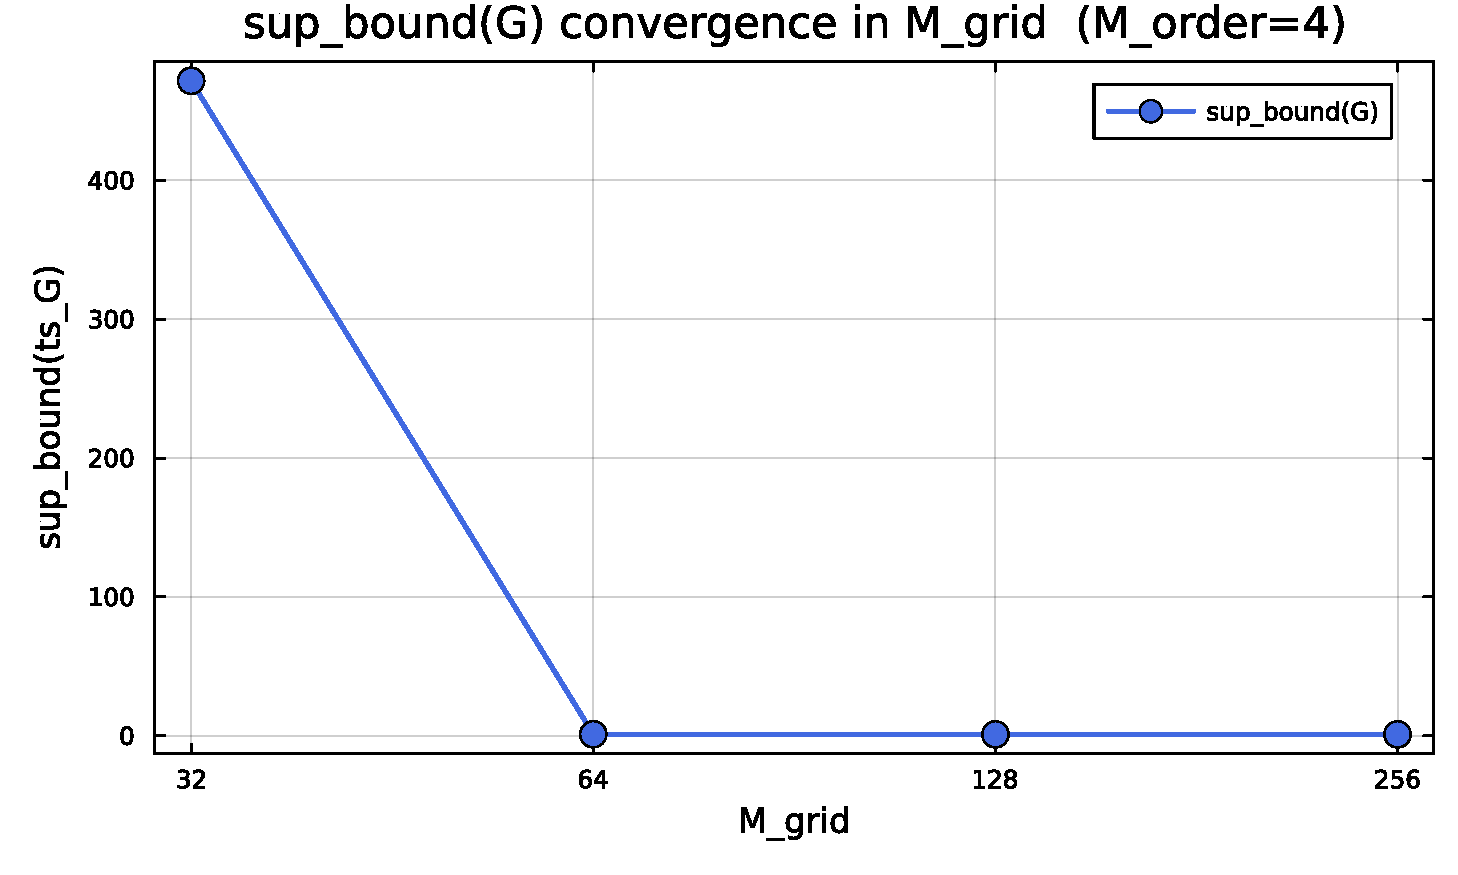
\includegraphics[width=\linewidth]{figures/fig_m3_3.pdf}
  \caption{T3.5: \texttt{sup\_bound}$(\texttt{ts\_G})$ vs.\ $M_{\mathrm{grid}}$
           for $y = 0.3\cos u + 0.15\cos 2u$, $M_{\mathrm{order}} = 4$.
           The bound decreases rapidly with grid refinement, converging to the
           true $\|G\|_\infty \approx 1.0$.
           ($M_{\mathrm{grid}} = 16$ is omitted: $D$ could not be certified positive
           at that resolution.)}
  \label{fig:m3_3}
\end{figure}

%% -------------------------------------------------------------------
\section{Summary}

\begin{table}[H]
\centering
\begin{tabular}{llcc}
\toprule
Test & Description & Assertions & Result \\
\midrule
T3.1 & $G^{(0)}$ ball contains prec=512 direct Arb eval at 64 grid pts & 1 &
  \textcolor{green!60!black}{\textbf{pass}} \\
T3.2 & $G^{(1)}$ ball contains analytic chain-rule value (prec=512) & 1 &
  \textcolor{green!60!black}{\textbf{pass}} \\
T3.3 & $G^{(2)}$ ball contains FD of analytic $G'$ ($h=10^{-50}$, prec=512) & 1 &
  \textcolor{green!60!black}{\textbf{pass}} \\
T3.4 & Analytical $G$ for $y = 0.1\cos u$ (128 pts + 3 special, contains) & 4 &
  \textcolor{green!60!black}{\textbf{pass}} \\
T3.5 & \texttt{sup\_bound}$(G)$ finite, positive, $< 10^6$ & 2 &
  \textcolor{green!60!black}{\textbf{pass}} \\
\midrule
\textbf{Total} & & \textbf{9} & \textcolor{green!60!black}{\textbf{9/9}} \\
\bottomrule
\end{tabular}
\caption{M3 test summary. All 9 assertions pass at 128-bit Arb precision.}
\end{table}

Milestone M3 is complete.  The \texttt{GDerivatives.jl} module provides:
\begin{itemize}
  \item \texttt{compute\_G\_taylor}: a certified \texttt{TaylorSeries} for
        $G = (1+\hat H[y_u])/D$ with rigorous full-vector \texttt{sup\_bounds}
        propagation through \texttt{inv\_series} (Fa\`a di Bruno on $1/x$)
        and product.
  \item A correctness guarantee for $G^{(m)}(u_j)$ at all grid points via
        Arb ball arithmetic.
  \item Convergence of \texttt{sup\_bound}$(G)$ to the true $\|G\|_\infty$
        as $M_{\mathrm{grid}} \to \infty$.
  \item A corrected \texttt{sqrt\_series} (missing Leibniz binomials fixed),
        which is required for all $m \ge 2$ derivative bounds to be correct.
\end{itemize}

The next milestone (M4) will use \texttt{ts\_G} to compute $\hat H[G]$ via
the DFT with aliasing control, completing the capillary-term bounds needed
for the certified residual estimate $\|R\|_{L^\infty} \le \varepsilon$.

\end{document}
